
%(BEGIN_QUESTION)
% Copyright 2011, Tony R. Kuphaldt, released under the Creative Commons Attribution License (v 1.0)
% This means you may do almost anything with this work of mine, so long as you give me proper credit

In this biogas generation system, cow manure is used as a feedstock to produce methane gas (CH$_{4}$), which is then used to fuel an engine to turn a generator and make electricity.  The waste heat from the engine is used to maintain the cascaded digesters (``reactors'' R-101 and R-102) at optimal temperatures for anaerobic bacteria to digest the manure and produce biogas (approximately 105 $^{o}$F):

$$\includegraphics[width=15.5cm]{i00664x01.eps}$$

Determine whether the manure liquid level process of reactor R-101 will naturally be {\it self-regulating}, {\it integrating}, or {\it runaway}.

\vskip 10pt

Assuming {\it reverse} control action for LIC-55, determine appropriate split-ranges for control valves LV-55a and LV-55b.  Assume we wish to avoid ``dead-heading'' the pump:

\begin{itemize}
\item{} LV-55a fully open at \underbar{\hskip 50pt} mA and fully closed at \underbar{\hskip 50pt} mA
\vskip 5pt
\item{} LV-55b fully open at \underbar{\hskip 50pt} mA and fully closed at \underbar{\hskip 50pt} mA
\end{itemize}

\vskip 10pt

Identify {\it two} different faults that could cause the engine to overheat, assuming the system has been working just fine for years:

\begin{itemize}
\item{} 
\vskip 5pt
\item{} 
\end{itemize}

\underbar{file i00664}
%(END_QUESTION)





%(BEGIN_ANSWER)

{\bf 2 points:} The liquid level process of reactor R-101 will naturally be {\bf integrating}.  Give full credit if the student answers ``self-regulating,'' because some level control processes are that.

\vskip 10pt

\begin{itemize}
\item{} {\bf 1 point for each answer:}
\item{} LV-55a fully open at \underbar{\bf 4} mA and fully closed at \underbar{\bf 20} mA
\item{} LV-55b fully open at \underbar{\bf 20} mA and fully closed at \underbar{\bf 4} mA
\end{itemize}

\vskip 10pt

{\bf 2 points for each of the two faults:}

\begin{itemize}
\item{} Coolant pump stopped
\item{} Fin-fan cooler fan motor stopped
\item{} TT-43 failed with low output signal
\item{} Leak in coolant piping
\item{} {\it Others . . . ?}
\end{itemize}

If a student writes more than two faults, grant points based on the {\it weakest} answer(s).  The idea here is to not grant credit for simply ``shotgunning'' with more than two answers, hoping at least two of them will be right.


%(END_ANSWER)





%(BEGIN_NOTES)

{\bf This question is intended for exams only and not worksheets!}.

%(END_NOTES)


